\clearpage
% \setcounter{page}{1}
\setcounter{figure}{0}
\setcounter{equation}{0}
% \setcounter{footnote}{0}
\setcounter{table}{0}
\setcounter{section}{0}
\appendix



\newpage
\begin{algorithm}[t]
\footnotesize
\caption{Algoritmo de InfiniPot-V}
\label{alg:infinipot_v}
\begin{algorithmic}[1]
\Require Flujo de video ${V}$, restricción de memoria $|M|$, tamaño objetivo de KV cache $|C|$, cantidad reciente de frames $r$, umbrales CV $\{\tau_1, \tau_2, \tau_3\}$, proporción TaR $\alpha \in [0,1]$, $f$ frames correspondientes a $|M|$ tokens, número de vision tokens por frame individual $p=|M|/f$ 
\Ensure KV cache comprimida $\{\tilde{K}_l, \tilde{V}_l\}_{l=1}^L$
\State Sea $C_{\text{TaR}} = \alpha|C|$ el presupuesto de selección de TaR
\State Sea $C_{\text{VaN}} = (1-\alpha)|C|$ el presupuesto de selección de VaN
\State Inicializar una KV cache vacía para cada capa $l \in \{1,\ldots,L\}$
\While{procesando el flujo de video ${V}$}
    \State Acumular embeddings KV hasta alcanzar $|M|$ 
    \For{each layer $l$}
        \State \textcolor{teal}{// Redundancia en el eje temporal (TaR)}
        \State Reshape $K_l$ into $K_{\text{recent},l} \in \mathbb{R}^{H \times r \times p \times D}$ and $K_{\text{past},l} \in \mathbb{R}^{H \times (f-r) \times p \times D}$
        \For{cada patch $(t,i,j)$ en frames pasados}
            \State $s(t,i,j) = -\frac{1}{r}\sum_{t'=1}^{r}\text{cos}(K_{\text{past},l}^{(t,i,j)}, K_{\text{recent},l}^{(t',i,j)})$
        \EndFor
        \State $\mathcal{I}_l \gets \text{TopK}(S_l, C_{\text{TaR}})$ \Comment{Seleccionar los tokens menos redundantes}
        
        \State \textcolor{teal}{// Value Norm (VaN) con Adaptive Pooling}
        \State $\text{VaN}_l \gets \|V_l\|_2$
        \State \textcolor{teal}{// Calcular CV para adaptive pooling}
        \State $\mu_l \gets \text{mean}(\text{VaN}_l)$
        \State $\sigma_l \gets \text{std}(\text{VaN}_l)$
        \State $\text{CV}_l \gets \sigma_l / \mu_l$
        \State \textcolor{teal}{// Determinar el tamaño de pooling usando la función de mapeo $g$}
\State $\text{pool\_size}_l \gets g(\text{CV}_l)$ \Comment{Usando los umbrales $\{\tau_1, \tau_2, \tau_3\}$}
\State \textbf{donde} $g(\text{CV}) = 
\begin{cases}
    7, & \text{if}\ \text{CV} < \tau_1 \\
    5, & \text{if}\ \tau_1 \leq \text{CV} < \tau_2 \\
    3, & \text{if}\ \tau_2 \leq \text{CV} < \tau_3 \\
    1, & \text{if}\ \text{CV} \geq \tau_3
\end{cases}$
        \State $\text{VaN}_{pool,l} \gets \text{AveragePool2d}(\text{VaN}_l, \text{pool\_size}_l)$
        
        \State \textcolor{teal}{// Combinar TaR y VaN priorizando los tokens seleccionados por TaR}
        \State $\text{VaN}_{pool,l}[\mathcal{I}_l] \gets \max(\text{VaN}_{pool,l})$ \Comment{Priorizar los tokens de TaR}
        \State $\mathcal{J}_l \gets \text{TopK}(\text{VaN}_{pool,l}, |C|)$ \Comment{Selección final de tokens}
        \State $\tilde{K}_l \gets K_l[:, \mathcal{J}_l, :]$, $\tilde{V}_l \gets V_l[:, \mathcal{J}_l, :]$ \Comment {Actualizar la KV cache de la capa con la KV cache comprimida}
    \EndFor
\EndWhile
\end{algorithmic}
\end{algorithm}


\begin{table}[t]
\centering
\small
\begin{tabular}{lcccccc}
\toprule
VideoMME  &\multicolumn{6}{c}{$|M| = \alpha |\text{TaR}| + (1-\alpha) |\text{VaN}|$, $|M| = 6\text{K}$} \\ \midrule
Qwen-2-VL-7B & $\alpha=0$ (VaN) & $\alpha=0.2$ & $\alpha=0.4$ & $\alpha=0.6$ & $\alpha=0.8$ & $\alpha=1$ (TaR) \\
\cmidrule(lr){1-7}
Short (-3 min) & 74.4 & 74.3 & 74.1 & 74.9 & 74.4 & 73.8 \\
Medium (3 - 30 min)  & 59.9 & 59.3 & 61.3 & 61.4 & 61.2 & 58.2 \\
Long (30 - 120 min)  & 51.9 & 51.0 & 52.4 & 53.1 & 53.4 & 53.2 \\ \cmidrule(lr){1-7}
Average  & 62.1 & 61.6 & 62.6 & \textbf{63.1} & \underline{63.0} & 61.7 \\
\midrule
LLaVA-Next-7B & $\alpha=0$ (VaN) & $\alpha=0.2$ & $\alpha=0.4$ & $\alpha=0.6$ & $\alpha=0.8$ & $\alpha=1$ (TaR) \\
\cmidrule(lr){1-7}
Short (-3 min)   & 69.8 & 69.8 & 72.0 & 71.1 & 71.9 & 68.8 \\
Medium (3 - 30 min)     & 59.3 & 59.3 & 59.2 & 58.7 & 57.7 & 57.3 \\
Long (30 - 120 min)    & 52.1 & 52.1 & 52.7 & 52.0 & 51.4 & 51.0 \\ \cmidrule(lr){1-7}
Average    & 60.4 & 60.4 & \textbf{61.3} & \underline{60.6} & 60.3 & 59.0 \\
\bottomrule
\end{tabular}
\vspace{2mm}
\caption{\textbf{TaR and VaN Combination Ratio}: Sweep over combination ratio $\alpha$ in TaR and VaN combination under a 6K memory budget ($|M|$) on VideoMME. $\alpha{=}0$ and $\alpha{=}1$ correspond to VaN-only and TaR-only, respectively. The best-performing configurations are shown in \textbf{bold}, while the second-best results are \underline{underlined}.}
\label{tab:alpha_sweep}
\vspace{-.15in}
\end{table}

\begin{table}[t]
\centering
\small
\begin{tabular}{lcccccccc}
\toprule
Qwen-2-VL-7B & \multicolumn{4}{c}{MLVU}            & \multicolumn{4}{c}{VideoMME}      \\
 \cmidrule(lr){1-1} \cmidrule(lr){2-5} \cmidrule(lr){6-9}
 $|M| = 6\text{K}$  & Holistic & Single & Multi & Avg. & Short & Medium & Long & Avg. \\
\midrule
$r=f\times0.125$        & 77.6 & 66.2 & 43.9 & \underline{63.1} & 68.7 & 57.3 & 51.0 & \textbf{59.0} \\
$r=f\times0.25$         & 77.8 & 67.1 & 43.5 & \textbf{63.4} & 68.0 & 57.2 & 51.1 & \underline{58.8} \\
$r=f\times0.50$          & 78.6 & 64.6 & 39.0 & 61.3 & 65.1 & 56.7 & 49.7 & 57.2 \\
\midrule
$|M|/|C|=0.75$   & 78.2 & 71.7 & 44.6 & \textbf{65.8} & 74.4 & 59.9 & 51.9 & \underline{62.1} \\
$|M|/|C|=0.50$   & 76.8 & 68.2 & 42.3 & \underline{63.3} & 74.1 & 60.3 & 52.9 & \textbf{62.4} \\
$|M|/|C|=0.25$   & 73.2 & 65.9 & 39.1 & 60.3 & 73.6 & 56.9 & 50.4 & 60.3 \\
\bottomrule
\end{tabular}
\vspace{2mm}
\caption{\textbf{Recent Frame and Compression Ratio Exploration}: \textbf{Top}: Sweep over recent frame numbers $r$ determined by multiplying various ratios ($0.125, 0.25, 0.5$) to $f$ (frame number corresponding to memory budget $|M|$) in TaR. \textbf{Bottom}: Performance under varying compression ratios $|M|/|C|$ across MLVU and VideoMME with \texttt{Qwen-2-VL-7B}. TaR performs best with $r\leq0.25$ and compression ratio $\geq0.5$. The highest values are shown in \textbf{bold}, with the second-highest \underline{underlined}.}
\label{tab:recent_compress_ratio}
\vspace{-.2in}
\end{table}

\section{InfiniPot-V Algorithm and Configuration}\label{appn:algorithm}


\subsection{Algorithm Description} Algorithm~\ref{alg:infinipot_v} presents the complete process of InfiniPot-V's cache control framework along with its compression formulation. InfiniPot-V processes video streams by continuously pre-filling and compressing the KV cache using two token selection strategies: Temporal-axis Redundancy (TaR) and Value Norm (VaN). For TaR, the algorithm splits video frames into recent frames (the latest $r$ frames) and past frames, then computes cosine similarities between corresponding patches to identify and remove redundant visual tokens. (Line 10)

For spatial semantic importance token selection, a layer-wise adaptive pooling mechanism based on VaN is employed. The pooling size is dynamically determined by the Coefficient of Variation (CV) of the VaN, (Line 18) where a higher CV indicates a sparser or more distinct feature distribution. Pre-computed model-specific CV thresholds $\{\tau_1, \tau_2, \tau_3\}$ determine pooling sizes from the set \{1,3,5,7\}, selecting larger windows for uniform (low CV) VaN distributions and smaller ones for sparse (high CV) VaN distributions (Line 21).

To integrate both criteria, TaR-selected tokens are prioritized by assigning them the maximum VaN score before the final token selection. Specifically, by setting $\text{VaN}_{pool,l}[\mathcal{I}_l] = \max(\text{VaN}_{pool,l})$ (Line 24) and then applying a TopK selection, the algorithm ensures that temporally distinctive tokens are preserved while allowing VaN to select additional tokens based on semantic importance.

\subsection{Hyper-Parameter Exploration}\label{appn:hyper_parameter} InfiniPot-V involves three main hyper-parameters: the TaR and VaN budget allocation ratio $\alpha$, the number of recent frames $r$ used in TaR, and the target compression size $C$ applied at each continual KV cache compression step. This section presents comparative experiments exploring each hyper-parameter.

\paragraph{TaR and VaN Budget Ratio ($\alpha$)} We compare the accuracy of offline video understanding (OVU) task across different values of $\alpha$, which determines the budget allocation between TaR and VaN under a fixed memory budget ($|M|=6\text{K}$), for both Qwen-2-VL-7B and LLaVA-Next-7B models. As shown in Tab.~\ref{tab:alpha_sweep}, performance peaks when $\alpha$ is between 0.4 and 0.6, outperforming the use of either VaN-only ($\alpha=0$) or TaR-only ($\alpha=1$). This confirms the effectiveness of our approach, which jointly considers both spatial and temporal dimensions for KV cache compression.

\paragraph{Recent Frames ($r$) and Compression Ratio ($|M|/|C|$)} Tab.~\ref{tab:recent_compress_ratio} presents exploration experiments for two key hyperparameters: the recent frames number $r$, which determines the proportion of recent frames within the memory budget in TaR, and the compression ratio $|M|/|C|$, which defines what proportion of the compression size $|C|$ to maintain relative to the memory budget $|M|$ in continual KV cache compression (CKV). 

For the recent frame number $r$ (Tab.~\ref{tab:recent_compress_ratio}, Top), we observe optimal performance on both MLVU and VideoMME benchmarks when $r \leq 0.25f$. Setting $r=0.5f$ results in an excessive number of frames being designated as the latest frames for temporal redundancy measurement, which limits the effectiveness of redundancy reduction. This limitation is reflected in the decreased performance metrics. (61.3 vs 63.4 in MLVU and 57.2 vs 59.0 in VideoMME) Note that the $r$ sweep experiments are conducted using TaR-only settings ($\alpha=1$).

For the compression ratio ($|M|/|C|$), we conduct comparative experiments across three ratios (0.75, 0.50, and 0.25). As shown in Tab.~\ref{tab:recent_compress_ratio} Bottom, an excessive compression ratio such as 0.25 in CKV results in noticeable performance degradation. These findings confirm that a ratio of 0.5 or higher represents an appropriate configuration for CKV.

Based on these explorations, we standardize the hyperparameter values at $\alpha=0.5$, $r=0.125$, and $|M|/|C|=0.75$ for all main experimental results when evaluating InfiniPot-V.


\section{Experimental Setting Details}\label{appn:exp}

\subsection{MLLMs Video Sampling Details.} For all benchmarks, we employ a consistent uniform frame sampling strategy to ensure maximized long video understanding performance across all settings. For Qwen-2-VL~\cite{Qwen2VL}, which supports dynamic image resizing based on the number of frames, we use the hyper-parameter configuration reported to yield the best performance in their original work: \texttt{FPS\_MAX\_FRAMES} = 768, \texttt{VIDEO\_MIN\_PIXEL} = ${128 \times 28 \times 28}$ and \texttt{VIDEO\_MAX\_PIXEL} = ${768 \times 28 \times 28}$. Although theoretically larger token budgets could be set, we adopt this configuration to match the optimal context length of 50K as reported in the original paper~\cite{Qwen2VL}, on top of which we applied KV cache compression. For LLaVA, we set the number of sampled frames to 128 to ensure it remained within the model’s trained context length (<32K). With this video sampling configuration, Qwen-2-VL~\cite{Qwen2VL} uses 384 frames with 130 tokens per frame, resulting in a total context length of 49,920 tokens, while LLaVA-Next~\cite{zhang2024llavanext-video} and LLaVA-OV~\cite{li2024llava} use 128 frames with 196 tokens per frame, yielding a total of 25,088 for offline long video inputs.

\subsection{Long Video Understanding Benchmark Details} 
\paragraph{Offline Video Understanding(OVU)} We evaluate our method on four multiple-choice based offline video question answering benchmarks: Video-MME~\cite{fu2024videomme}, MLVU~\cite{MLVU}, EgoSchema~\cite{mangalam2023egoschema}, and LongVideoBench~\cite{wu2024longvideobench}. For MLVU and EgoSchema, we use the development sets for evaluation.

For Video-MME, we report results without subtitles version. This is because prepending subtitles for all video frames as a single context block directly before the question represents an unrealistic setting that is incompatible with streaming scenarios, where subtitles are typically unavailable during real-time video processing and would not be accessible as complete context in advance.

\paragraph{Streaming Video Understanding (SVU)} For SVU evaluation, we use two benchmarks: RVS-Ego and EVS-Movie~\cite{zhang2024flashvstream}. RVS-Ego is constructed from 10 videos from the Ego4D~\cite{Grauman_2022_CVPR} dataset, while RVS-Movie uses 22 long videos from MovieNet~\cite{huang2020movienet}. Each benchmark consists of a QA set containing open-ended generation questions and their corresponding timestamps indicating when each question should be presented during video streaming.

The evaluation process works as follows: during CKV processing, when the video stream reaches the timestamp of a given question sample, we present the question and generate an answer based on the compressed KV cache accumulated up to that point. The generated answers are then compared against ground-truth answers using \texttt{GPT-3.5-turbo-0125} to produce accuracy and score metrics.

\subsection{Baseline Settings}
\paragraph{Input Video Compression (IVC) Details.}
For the comparison with Input Video Compression (IVC) methods in Tab.~\ref{tab:ic_cache} and ~\ref{tab:full_ivc}, we implement LongVU~\cite{shen2024longvu} and DyCoke~\cite{tao2024dycokedynamiccompressiontokens} as follows: For \textbf{LongVU}, we apply Spatial Token Compression (STC) every 8 frames as specified in the original paper. STC compresses vision token embeddings by identifying temporally redundant patches using cosine similarity between patches. We adjust the similarity threshold to control the compression rate while maintaining the original methodology. For \textbf{DyCoke}, we implement Token Temporal Merging (TTM) which, similar to LongVU, compresses vision encoder output features. TTM calculates cosine similarity between patches in adjacent frames to eliminate redundant patch embeddings. Following the original paper, we process compression every 4 frames and adjust the similarity threshold to control compression rates.

For fair comparison in the Continual KV cache compression (CKV) framework in Tab.~\ref{tab:ic_cache}, we adapt both methods to work within memory constraint $|M|$. Specifically, we compress each input video stream to size $|C|$ and implement sliding window attention~\cite{Beltagy2020Longformer} to evict older KV cache entries once the cache size reaches the predefined memory limit ($|M|$). This adaptation ensures all methods operate under identical memory constraints for a fair comparison with InfiniPot-V. For benchmark comparing InfiniPot-V with IVC methods that use full vision encoding without cache compression, see Tab.~\ref{tab:full_ivc}.

\paragraph{KV Cache Compression (KVC) Details.} In Fig.~\ref{fig:cache_compression}, we compare three KV cache compression methods within Continual KV cache compression (CKV). First, \textbf{Uniform Select}, inspired by uniform video sampling approaches, selects frames at regular intervals and retains all KV cache tokens corresponding to those frames. For \textbf{SnapKV}~\cite{li2024snapkv}, we follow the original method configuration under the CKV process, using the last 32 tokens of the given budget $|M|$ tokens as an observation window ($w$) to calculate attention scores for token selection (see Eq.~\ref{eq:importance-future} in Appendix.~\ref{appn:prelim}). Additionally, we apply 1D pooling with a kernel size of 7 to these scores, as done in the original implementation\footnote{https://github.com/FasterDecoding/SnapKV}. For \textbf{InfiniPot}~\cite{kim-etal-2024-infinipot}, we design a proxy prompt for video compression: "Provide a detailed description of this video." This prompt is utilized in the CaP method to generate attention scores and apply KV cache compression. Detailed experimental results are provided in Tab.~\ref{tab:full_table}.

\paragraph{FastV Hyper-Parameter Settings.} To provide additional performance comparison with compression methods specialized for MLLMs, we also include performance comparisons with FastV~\cite{chen2024image} in Tab.\ref{tab:full_table}. FastV requires two hyper-parameters, $L$ and $R$, which specify the layer where token pruning begins and the percentage of tokens to prune. For a fair comparison, we adjust the $R$ of FastV to ensure that the total number of KV cache entries across layers matches the total entry count of other baselines that maintain the same number of KV-cache entries across each layer.  Specifically, for Qwen-2-VL, the $(L, R)$ pairs corresponding to memory budgets of 3K, and 6K are set to (2, 2.8\%) and (2, 5.8\%) respectively.

\subsection{Positional Encoding Details.} MLLM backbone LLMs utilize positional encoding to differentiate vision token positions. LLaVA-Next~\cite{zhang2024llavanext-video} and LLaVA-OV~\cite{li2024llava} use standard 1D RoPE~\cite{su2023roformerenhancedtransformerrotary}, while Qwen-2-VL~\cite{Qwen2VL} employs 3D RoPE for multimodal encoding. For Offline Video Understanding(OVU), we apply KV cache compression after positional encoding (i.e., Post RoPE). However, Streaming Video Understanding(SVU) presents a challenge: continuous video stream processing can exceed the model's maximum positional range. For example, in LLaVA models with 196 tokens per frame, streaming more than 6 minutes of video at 0.5 FPS exceeds the 32K context window (note that RVS-Ego and RVS-Movie average over 60 minutes). 

To address this, we adopt strategies from InfiniPot~\cite{kim-etal-2024-infinipot} and ReKV~\cite{Shangzhe2025streaming}, re-ordering positional indices to fit within the memory budget $|M|$ at each CKV step. Specifically, we cache the pre-positional encoded KV's hidden states and re-assign positional indices during decoding, ensuring they never exceed $|M|$ position regardless of video length. While this enables SVU for arbitrarily long videos, it discards the original positional information of vision tokens. In particular, additional handling is required for Qwen-2-VL’s 3D RoPE. Developing methods that preserve the original spatial and temporal position encoding while supporting streaming video lengths beyond the model’s positional capacity remains an open direction for future work.


% The model code was implemented based on the official repositories of LLaVA-Next~\cite{zhang2024llavanext-video}~\footnote{https://github.com/LLaVA-VL/LLaVA-NeXT} and Qwen-2.5-VL~\footnote{https://github.com/QwenLM/Qwen2.5-VL}.


\begin{figure*}[t]
\centerline{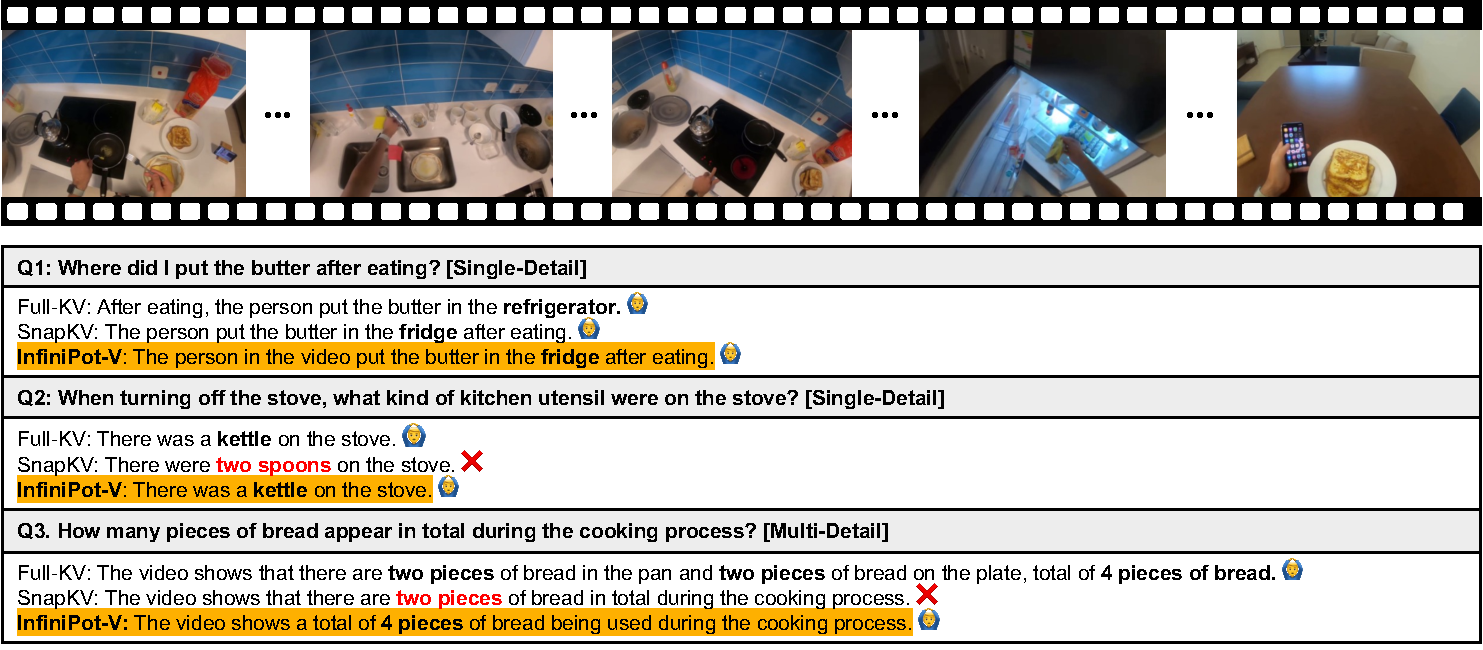
\includegraphics[width=1\textwidth]{Figures/appn_fig1.pdf}}
\caption{\textbf{Qualitative Results of Multi-Turn Conversation}: Full-KV uses 16K cache while InfiniPot-V and SnapKV employ 3K compressed KV cache. SnapKV performs query-guided cache compression based on Q1 before proceeding with multi-turn conversation. The video sample is from the MLVU ego reasoning subtask, using the \texttt{Qwen-2-VL-7B model}. 128 frame sampling is used.}\label{fig:multi_turn}
\vspace{-.2in}
\end{figure*}

\section{Multi-Turn Video Understanding Analysis}\label{appn:multi_turn}
Fig.~\ref{fig:multi_turn} presents a qualitative comparison between query-dependent (SnapKV)\cite{li2024snapkv} and query-agnostic (InfiniPot-V) KV cache compression approaches in multi-turn conversations with streaming video input. When SnapKV performs compression based on Q1, it generates answers almost identical to the Full KV cache for that specific query (Q1), answering that the butter was placed in the refrigerator. However, this query-guided compression strategy reveals significant limitations when handling different types of queries (Q2, Q3) about the same video content. Specifically, SnapKV makes critical errors in subsequent queries - misidentifying a kettle as "two spoons" in Q2 and incorrectly counting the total number of bread pieces in Q3.

In contrast, InfiniPot-V maintains accurate answers consistently across all three queries using the same 3K compressed KV cache. It correctly identifies that the butter was placed in the fridge (Q1), recognizes the kettle on the stove (Q2), and counts all 4 pieces of bread throughout the cooking process (Q3), demonstrating the effectiveness of query-agnostic compression for multi-turn streaming video scenarios.

\section{Why Query-Agnostic KV Cache Compression Matters for SVU?}\label{appn:query_agnostic}

In this section, we provide a detailed analysis of why query-agnostic compression is essential for Streaming Video Understanding (SVU), building upon the requirements discussed in Sec.~\ref{sec:background}. To demonstrate how these SVU-specific constraints impact existing KV cache compression methods, we present a case study across three representative scenarios.

% In this section, we discuss the core requirements of Streaming Video Understanding (SVU) from the perspective of KV cache compression, with particular emphasis on analyzing why \textit{query-agnostic} compression is essential as discussed in Sec.~\ref{sec:background}. 

\subsection{Preliminary: Attention-based KV Cache Compression}\label{appn:prelim}

Eviction-based KV cache compression reduces cache size by removing tokens with the lowest importance scores.
Employing attention scores for computing token importance scores is the predominant approach in previous methods~\cite{li2024snapkv,chen2024image,fu2024headkv,hooper2024squeezed}.

In methods such as SnapKV~\cite{li2024snapkv}, the importance scores $u_t$ of a token $x_t$ are computed by aggregating attention scores from the last $w$ tokens (i.e., observation window) which contain the user instruction:
\vspace{-.1in}
\begin{equation}
u_t = \sum_{i=N-w}^{N} \text{Attn}(x_{i} \rightarrow x_{t}),
\label{eq:importance-future}
\end{equation}
where $N$ is the current sequence length.
Using these scores, the KV cache is compressed by retaining the top-$M$ tokens with the highest aggregated attention scores.
Here, $M$ defines the memory budget: $\mathcal{I} = \text{TopK}(u, M)$ and $u = [u_1, \cdots, u_N]$ indicates the importance scores of all tokens.
The compressed Key and Value caches are then formed by extracting tokens at indices $\mathcal{I}$:
\begin{equation}
\tilde{K} = K[:, \mathcal{I}, :], \quad \tilde{V} = V[:, \mathcal{I}, :]
\label{eq:cache-compression}
\end{equation}
where $K, V \in \mathbb{R}^{H \times N \times D}$ are the uncompressed Key and Value caches with $H$ heads, $N$ tokens, and per-head dimension $D$. 
This approach has two characteristics: (1) it requires computing the full KV cache for all tokens before compression, and (2) it requires the user query to be present at the end of the context. We refer to these approaches as \textit{query-guided} or \textit{attention-based} cache compression methods.\footnote{Throughout this paper, "query" refers to the user's instruction or question related to the given video.}

\begin{figure}
    \centering
    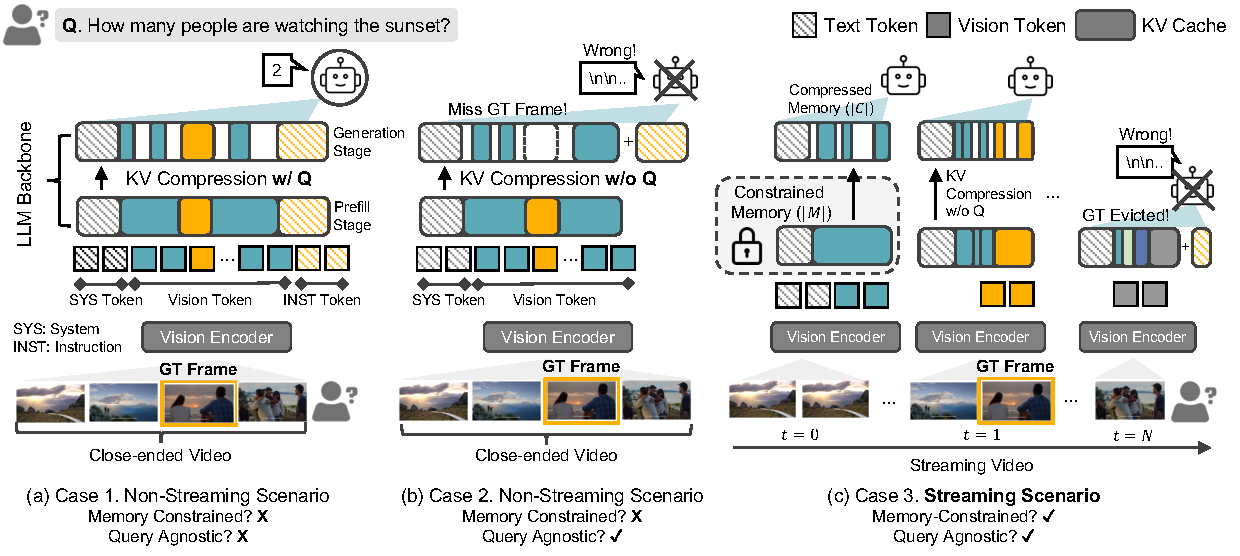
\includegraphics[width=1\linewidth]{Figures/appn_fig2.pdf}
\caption{\textbf{KV Cache Compression Case Study with SVU}: Illustration of cache control strategies under three conditions, differing in the presence of two core requirements for Streaming Video Understanding (SVU): memory constrained (MC) and query agnostic (QA). (a) Case 1: Query-guided compression retains relevant (GT) frames for accurate responses. (b) Case 2: Without query guidance, compression fails to preserve critical frames, resulting in inaccurate responses. (c) \textbf{Case 3} \textbf{(Streaming scenario)}: In streaming video processing, where frames arrive continuously, continual KV cache compression (CKV) is necessary, but queries are unavailable during compression.}
\label{fig:case_study}
\vspace{-2mm}
\end{figure}


\subsection{Case Study: Towards Streaming Video Understanding with CKV}\label{appn:case_study}

To investigate the applicability of attention-based KV cache compression methods to streaming video understanding, we examine three cache control strategies (Fig.~\ref{fig:case_study}).

\begin{wraptable}{r}{0.5\columnwidth}
\scriptsize
\begin{tabular}{c|c|c|cc@{}}
\toprule
Case & \makecell{$x_t$ Attention \\ Scoring} & \makecell{Prefill \\ $|M|$} & \makecell{Gen. \\ $|M|$ = 3K} & \makecell{Gen. \\ $|M|$ = 6K} \\ 
\midrule
Full KV & n/a & 25K & \multicolumn{2}{c}{68.75 (↑)} \\ \midrule
Case 1 & $\text{Attn}(q \rightarrow x_{t})$ & 25K & 68.01 & 68.40 \\ \midrule
\multirow{3}{*}{Case 2} & $\text{Attn}(q' \rightarrow x_{t})$ & \multirow{3}{*}{25K} & 60.35 & 63.42 \\ 
                        & $\text{Attn}(q'' \rightarrow x_{t})$ & & 60.60 & 63.50 \\ 
                        & $\text{Attn}(q_v \rightarrow x_{t})$ & & 60.32 & 62.28 \\ \midrule
\textbf{Case 3} & $\text{Attn}(q_v \rightarrow x_{t})$ & 3K/6K & 57.55 & 59.98 \\ 
\bottomrule
\end{tabular}
\caption{\textbf{Case study of Attention Scoring}: conducted on MLVU benchmark with \texttt{LLaVA-Next-Video-7B}. Note that memory-constrained setting (Case 3) shares the same budget during prefill and generation stages.}\label{tab:case_study}
\vspace{-.15in}

\end{wraptable}

\paragraph{Case 1.} Recent KV cache compression methods~\cite{li2024snapkv,fu2024headkv} assume full access to context and queries at compression time, as shown in Fig.~\ref{fig:case_study}(a). In this memory-unconstrained setting, the model observes the full input before compression. Previous works~\cite{li2024snapkv} have demonstrated that attention scores effectively identify query-relevant tokens KV cache (orange box corresponding to GT Frame in Fig.~\ref{fig:case_study}(a)), enabling compression that retains critical information while discarding less important tokens. As shown in Tab.~\ref{tab:case_study}, this approach maintains performance comparable to the uncompressed cache setup (68.01 vs 68.75) at the cost of large memory usage at compression, detailed in Fig.~\ref{fig:background}.



\paragraph{Case 2.} Fig.~\ref{fig:case_study}(b) illustrates how attention-based cache compression fails when user queries are unavailable during compression.
Under this scenario, although the memory budget is assumed unconstrained, the KV cache is compressed without consideration of (future) queries, causing important visual tokens (orange tokens cache corresponding to the GT Frame) lost during compression.
To quantify this degradation and explore alternatives, we test compression with generic queries ($q'$: "What is happening in this video?", $q'':$"What are the key events in this video?") and the last vision tokens ($q_v$) for importance scoring:

\begin{equation}
u^{\text{alt}}_t = \text{Attn}(q_{\text{alt}} \rightarrow x_t), \quad 
q_{\text{alt}} \in \{q', q'', q_v\}
\label{eq:alternative-importance}
\end{equation}

Tab.~\ref{tab:case_study} and Fig.~\ref{fig:case_study}(a) show that these alternatives significantly degrade performance (60.32 vs 68.75), even with unconstrained memory.

\paragraph{Case 3: Streaming Scenario.} Beyond the query-agnostic challenge in Case 2, deploying streaming video understanding on resource-constrained devices requires fixed memory usage for the KV cache.
For input video streams, these constraints necessitate continual compression when new frames arrive and memory capacity is reached, as shown in Fig.~\ref{fig:case_study}(c).
To evaluate this scenario, we use the query-agnostic approach from Case 2 with vision tokens ($q_v$) for importance scoring, while compressing the KV cache whenever memory limits are reached.
As shown in Tab.~\ref{tab:case_study}, this combined constraint further degrades performance (57.55 vs 60.32), highlighting the challenge of preserving key information under both query-agnostic and memory-constrained settings.

This case study reveals two key challenges for KV cache compression in streaming video: 1) the need for \textit{query-agnostic compression} due to continuous incoming video, and 2) the requirement to maintain \textit{fixed memory constraints}. These challenges cause significant performance drops in previous methods~\cite{li2024snapkv,kim-etal-2024-infinipot,chen2024image}, motivating Continual KV cache compression (CKV) specifically designed for memory-constrained streaming video.


% \usepackage{caption}   % for \captionof

\begin{table}[t]
  \centering
  % left = figure
  \begin{minipage}[t]{0.5\textwidth}
    \vspace{0pt}                 % makes the [t] stick
    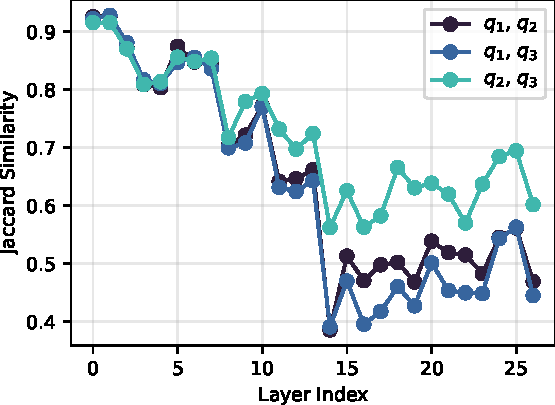
\includegraphics[width=0.95\textwidth]{Figures/appn_fig3.pdf}
    \vspace{0.5mm}
    \captionof{figure}{\textbf{Jaccard Similarity between KV Caches}: Compare KV cache sets selected by different queries ($q_1,q_2,q_3$) across layers.}
    \label{fig:jac_sim}
  \end{minipage}%
  \hfill
  % right = table
  \begin{minipage}[t]{0.45\textwidth}
    \vspace{2pt}
    \resizebox{\textwidth}{!}{%
      \begin{tabular}{c|cc|cc}
        \toprule
        Context & \multicolumn{2}{c|}{Case 1, 2} & \multicolumn{2}{c}{Case 3 (Ours)} \\
        Length & Mem (GB) & TTFT (s) & Mem (GB) & TTFT (s) \\ 
        \midrule
        5K    & 21.29 & 0.98 & 20.93 & 1.08 \\
        25K   & 33.76 & 1.21 & 21.60 & 1.12 \\
        50K   & 58.55 & 2.12 & 22.16 & 1.17 \\
        100K  & 79.38 & 3.27 & 22.85 & 1.20 \\
        \bottomrule
      \end{tabular}%
    }
    \vspace{2mm}
    \captionof{table}{\textbf{Peak GPU Memory and TTFT}: Comparison of peak memory usage and Time-To-First-Token(TTFT) across different context lengths for memory-unconstrained (Case 1, 2) and memory-constrained (Case 3) approaches.}
    \label{tab:memory_ttft}
  \end{minipage}
  \vspace{-.2in}
\end{table}


\paragraph{Attention Scoring Analysis} We further analyze the query-dependent nature of attention-based KV cache compression using the VideoMME benchmark. To investigate why performance varies with different queries, we compute the Jaccard similarity between token sets selected for different queries across layers using attention scores at each layer. For this analysis, $q_1, q_2, q_3$ represent three distinct questions associated with the same video sample in the VideoMME benchmark. As shown in Fig.~\ref{fig:jac_sim}, the similarity between token sets decreases significantly in the middle-to-late layers, dropping to around 0.4. This indicates that each query selects a different set of tokens, particularly in deeper layers. This analysis highlights that attention-based scoring methods inherently select query-specific tokens, explaining the performance degradation when query information is unavailable or changes during streaming video scenarios.

\section{Memory and Latency Measurement Results}\label{appn:memory_latency}

Table~\ref{tab:memory_ttft} presents measurements of peak memory consumption and Time-To-First-Token (TTFT) during the prefill stage, conducted on a single NVIDIA A100-80GB GPU using PyTorch. The experiments averaged over five runs with three warmup iterations, compare the performance of memory-unconstrained (Case 1, 2) and memory-constrained (Case 3) approaches across various context lengths. For memory-unconstrained methods, we observe a linear growth in memory requirements, escalating from 21.29 GB at 5K tokens to 79.38 GB at 100K tokens, accompanied by a proportional increase in TTFT from 0.98 to 3.27 seconds.

Our memory-constrained continual KV cache compression (Case 3) exhibits remarkably different behavior. Despite the increasing context length, the peak memory usage shows only minimal growth, rising modestly from 20.93 GB at 5K tokens to 22.85 GB at 100K tokens. Similarly, the TTFT remains relatively stable, increasing from 1.08 to 1.20 seconds across the same range. These detailed measurements demonstrate that our approach effectively maintains near-constant resource utilization while processing extended video frames.

\section{Trabajo relacionado}\label{sec:related}

\subsection{MLLMs para Long Video Understanding}
Los avances recientes en MLLMs de contexto largo han atraído una atención significativa. Entre los ejemplos destacados se encuentran Gemini-2.0~\cite{google2024cgemini-2.0}, con soporte para streaming video; LongVILA~\cite{Chen2025longvila}, capaz de manejar hasta 6,000 frames de video; LLaVA-Next-Video~\cite{zhang2024llavanext-video}, que aprovecha datos sintéticos de instrucciones de alta calidad; y Qwen-2-VL~\cite{Qwen2VL}, que permite análisis de videos de una hora mediante multimodal RoPE.

\subsection{Input-Vision Compression (IVC)}
Para abordar las demandas computacionales del procesamiento de videos de larga duración, se han propuesto varios enfoques para comprimir información visual redundante antes de que ingrese al backbone LLM. 

LongVU~\cite{shen2024longvu} adopta muestreo de frames de entrada dependiente de la consulta y eliminación de píxeles redundantes para fine-grained video understanding, pero el vision encoding de dos torres produce alta latencia durante el muestreo de entrada, lo que lo vuelve impráctico para escenarios de streaming. Además, este enfoque requiere entrenar modelos especializados para operar de la manera propuesta, limitando su aplicabilidad a modelos preentrenados existentes. 

DyCoke~\cite{tao2024dycokedynamiccompressiontokens} reduce redundancias entre frames adyacentes a nivel del video de entrada y actualiza dinámicamente tokens relacionados con la consulta en la KV cache desde almacenamiento externo. Slow-Fast-LLaVA-1.5~\cite{xu2025slowfastllava15familytokenefficientvideo} propone dividir el procesamiento del video de entrada en trayectorias slow y fast separadas, usando distintos métodos de proyección para reducir los input vision tokens. Sin embargo, este enfoque todavía sufre la limitación de requerir que todos los input vision tokens se procesen simultáneamente y necesita entrenamiento adicional del modelo.

\subsection{KV Cache Compression (KVC)}
Comprender el contexto largo en MLLMs exige un control eficiente de la KV cache para manejar el crecimiento de memoria y la sobrecarga de latencia. Los métodos de compresión de KV cache pueden clasificarse, en términos generales, en enfoques dependientes e independientes de la consulta.

\paragraph{Compresión de KV cache dependiente de la consulta.}
Métodos como SnapKV~\cite{li2024snapkv}, H2O~\cite{zhang2023ho}, HeadKV~\cite{fu2024headkv} y ThinK~\cite{xu2025think} aprovechan puntajes de atención consulta-contexto para identificar entradas KV cruciales, pero requieren que el contexto completo pase por prefill antes de la compresión, lo que los vuelve imprácticos bajo restricciones de memoria. En el dominio multimodal, FastV~\cite{chen2024image} acelera el prefill podando vision tokens en ciertas capas según sus puntajes de atención desde el token final de consulta.
SparseVLM~\cite{zhang2024sparsevlm} selecciona visual tokens relevantes para las consultas del usuario mediante cross-attention. En general, los métodos dependientes de la consulta comprimen eficazmente el contexto, pero tienen dificultades para manejar consultas diversas sobre un contexto ya comprimido~\cite{tang2025razorattention}. ReKV~\cite{Shangzhe2025streaming} aborda escenarios de streaming video descargando la KV cache relacionada con video a memoria CPU y recuperando bajo demanda entradas de cache dependientes de la consulta. Este enfoque depende de almacenamiento externo y sufre sobrecarga de transferencia de datos, lo que lo vuelve inadecuado para streaming video understanding con memoria restringida.

\paragraph{Compresión de KV cache independiente de la consulta.}
Trabajos recientes persiguen la compresión de KV cache independiente de la consulta para eliminar la dependencia de consultas futuras~\cite{ge2024model,devoto2024simple,hooper2024squeezed, kim2025kvzipqueryagnostickvcache, corallo2025ragtaskawarekvcache,park2025keydiffkeysimilaritybasedkv}.
En particular, SqueezedAttention~\cite{hooper2024squeezed} usa clustering basado en keys, pero requiere encoding de contexto completo, lo que limita su aplicabilidad en escenarios con memoria restringida.
InfiniPot~\cite{kim-etal-2024-infinipot} comprime el contexto aproximando posibles consultas del usuario mediante un proxy prompt específico de la tarea, pero su prompt fijo restringe la flexibilidad. En el dominio de visión, HiRED~\cite{arif2024hired} y FasterVLM~\cite{zhang2024fastervlm} utilizan puntajes de atención del token [CLS] para las decisiones de compresión. Sin embargo, su dependencia de tokens especiales restringe su aplicación a MLLMs recientes que carecen de tales tokens~\cite{qwen2.5,zhang2024llavanext-video}, limitando su aplicabilidad más amplia.


\section{Experimental Results Data}

\begin{table*}[t!]
    \centering
    \resizebox{\textwidth}{!}
    {
    \begin{tabular}{c|cc|c|c|c|cccc|cccc|c|c}
    \toprule
    \multirow{2}{*}{\rotatebox[origin=c]{90}{Case}}& \multicolumn{2}{c|}{Streaming} & Compression & Prefill & Decoding & \multicolumn{4}{c|}{VideoMME} & \multicolumn{4}{c|}{MLVU} & \multirow{2}{*}{LVB} & \multirow{2}{*}{Avg.} \\
    & MC & QA & Method & Budget & Budget & Short & Medium & Long & Avg. & Holistic & Single & Multi & Avg. & & \\
    \midrule
    \multicolumn{16}{c}{\textbf{Qwen-2-VL-7B}} \\
    \midrule
    & - & - & Full KV & 50K & 50K & 74.68 & 62.11 & 55.00 & 63.93 & 76.34 & 73.91 & 43.29 & 65.85 & 58.77 & 62.85 \\
    \cmidrule{1-16}
    \multirow{4}{*}{\rotatebox[origin=c]{90}{Case 1}} & \multirow{4}{*}{\ding{55}} & \multirow{4}{*}{\ding{55}} & FastV~\cite{chen2024image} & \multicolumn{2}{c|}{48/3K~($R=2.8$)} & 54.11 & 50.11 & 48.67 & 50.96 & 69.59 & 59.40 & 33.84 & 55.01 & 47.94 & 51.30 \\
    & & & ($L=2$) & \multicolumn{2}{c|}{48/6K~($R=5.8$)} & 59.67 & 54.55 & 50.78 & 55.00 & 72.00 & 64.08 & 33.47 & 57.60 & 50.53 & 54.38 \\
    \cmidrule{4-16}
    & & & \multirow{2}{*}{SnapKV~\cite{li2024snapkv}} & 50K & 3K & 74.00 & 61.00 & 54.22 & 63.07 & 77.08 & 67.49 & 39.07 & 62.11 & 59.06 & 61.42 \\
    & & & & 50K & 6K & 74.22 & 60.55 & 54.33 & 63.03 & 77.59 & 73.91 & 42.90 & 66.10 & 58.80 & 62.64 \\
    \midrule
    \multirow{4}{*}{\rotatebox[origin=c]{90}{Case 2}} & \multirow{4}{*}{\ding{55}} & \multirow{4}{*}{\ding{51}} & \multirow{2}{*}{Uniform} & 50K & 3K & 70.33 & 54.67 & 49.55 & 58.18 & 72.29 & 59.06 & 33.51 & 55.54 & 59.80 & 57.84 \\
    & & & & 50K & 6K & 72.00 & 58.78 & 52.11 & 60.96 & 77.08 & 67.49 & 39.07 & 62.11 & 59.11 & 60.73 \\
    \cmidrule{4-16}
    & & & \multirow{2}{*}{SnapKV$^\dag$} & 50K & 3K & 69.00 & 54.00 & 50.67 & 57.89 & 75.88 & 63.48 & 35.35 & 58.99 & 56.70 & 57.86 \\
    & & & & 50K & 6K & 72.11 & 57.56 & 52.22 & 60.63 & 76.46 & 66.43 & 36.22 & 60.66 & 56.72 & 59.34 \\
    \midrule
    % \multirow{12}{*}{\rotatebox[origin=c]{90}{Case 3}} & \multirow{12}{*}{\ding{51}} & \multirow{12}{*}{\ding{51}} & \multirow{3}{*}{Uniform} & 3K & 3K & 66.00 & 52.44 & 48.00 & 55.48 & 72.54 & 59.00 & 33.51 & 55.59 & 55.21 & 55.43 \\
    % & & & & 6K & 6K & 72.33 & 53.33 & 48.67 & 58.11 & 72.55 & 62.19 & 33.67 & 57.00 & 55.82 & 56.98 \\
    % & & & & 12K & 12K & 74.00 & 55.33 & 51.44 & 60.26 & 75.94 & 65.53 & 37.01 & 60.36 & 57.91 & 59.51 \\
    % \cmidrule{4-16}
    \multirow{16}{*}{\rotatebox[origin=c]{90}{Case 3 (CKV)}} & \multirow{16}{*}{\ding{51}} & \multirow{16}{*}{\ding{51}} & \multirow{4}{*}{Uniform} & 3K & 3K & 66.00 & 52.44 & 48.00 & 55.48 & 72.54 & 59.00 & 33.51 & 55.59 & 55.21 & 55.43 \\
    & & & & 6K & 6K & 72.33 & 53.33 & 48.67 & 58.11 & 72.55 & 62.19 & 33.67 & 57.00 & 55.82 & 56.98 \\
    & & & & 12K & 12K & 74.00 & 55.33 & 51.44 & 60.26 & 75.94 & 65.53 & 37.01 & 60.36 & 57.91 & 59.51 \\
    & & & & 24K & 24K & 74.22 & 59.22 & 53.22 & 62.22 & 77.22 & 71.10 & 40.78 & 64.18 & 58.60 & 61.67 \\
    \cmidrule{4-16}
    
    & & & \multirow{4}{*}{SnapKV$^\ddag$} & 3K & 3K & 66.67 & 52.22 & 49.89 & 56.26 & 75.88 & 63.48 & 35.35 & 58.99 & 54.91 & 56.72 \\
    & & & & 6K & 6K & 72.00 & 55.33 & 51.33 & 59.55 & 76.46 & 66.43 & 36.22 & 60.66 & 55.15 & 58.45 \\
    & & & & 12K & 12K & 74.44 & 58.89 & 52.89 & 62.07 & 75.71 & 68.61 & 35.98 & 61.31 & 56.89 & 60.09 \\
    & & & & 24K & 24K & 74.22 & 61.00 & 53.78 & 63.00 & 77.66 & 71.82 & 39.90 & 64.37 & 59.09 & 62.15 \\
    \cmidrule{4-16}
    
    & & & \multirow{4}{*}{InfiniPot~\cite{kim-etal-2024-infinipot}}& 3K & 3K & 67.11 & 54.55 & 51.00 & 57.55 & 74.94 & 61.80 & 36.60 & 58.36 & 54.00 & 56.64 \\
    & & & & 6K & 6K & 72.89 & 57.33 & 51.33 & 60.52 & 75.02 & 63.18 & 37.09 & 59.11 & 54.64 & 58.09 \\
    & & & & 12K & 12K & 74.00 & 57.78 & 53.22 & 61.67 & 74.46 & 66.46 & 38.30 & 60.70 & 56.94 & 59.77 \\
    & & & & 24K & 24K & 74.22 & 60.55 & 53.56 & 62.78 & 76.03 & 71.11 & 40.29 & 63.71 & 57.85 & 61.44 \\
    
    \cmidrule{4-16}
    \mscellf & & & & 3K & 3K & 73.89 & 57.78 & 51.78 & 61.11 & 77.73 & 70.38 & 43.15 & 64.70 & 57.64 & 61.15 \\
    \mscells & & & & 6K & 6K & 74.11 & 60.78 & 53.44 & 62.78 & 77.16 & 72.31 & 44.75 & 65.82 & 58.40 & 62.33 \\
    \mscellt & & & & 12K & 12K & 74.22 & 62.68 & 53.89 & 63.59 & 76.90 & 73.41 & 43.97 & 65.99 & 59.18 & 62.92 \\
    \mscellfo & & & \multirow{-4}{*}{\textbf{InfiniPot-V}} & 24K & 24K & 74.22 & 63.22 & 53.11 & 63.52 & 76.91 & 73.97 & 42.18 & 65.73 & 58.94 & 62.73 \\
    
    \midrule
    \multicolumn{16}{c}{\textbf{LLaVA-Next-Video-7B}} \\
    \midrule
    & - & - & Full KV & 25K & 25K & 74.33 & 60.11 & 54.11 & 62.85 & 80.60 & 73.73 & 49.43 & 68.75 & 63.55 & 65.05 \\
    \midrule
    \multirow{4}{*}{\rotatebox[origin=c]{90}{Case 1}} & \multirow{4}{*}{\ding{55}} & \multirow{4}{*}{\ding{55}} & \multirow{2}{*}{Uniform} & 25K & 3K & 74.33 & 62.33 & 55.00 & 63.89 & 80.29 & 72.38 & 49.19 & 68.01 & 62.35 & 64.75 \\
    & & & & 25K & 6K & 73.89 & 62.00 & 54.78 & 63.56 & 80.66 & 72.25 & 49.62 & 68.19 & 62.55 & 64.76 \\
    \cmidrule{4-16}
    & & & \multirow{2}{*}{SnapKV~\cite{li2024snapkv}} & 25K & 3K & 74.44 & 59.89 & 53.78 & 62.70 & 80.41 & 73.01 & 49.67 & 68.46 & 62.34 & 64.50 \\
    & & & & 25K & 6K & 74.44 & 60.11 & 53.78 & 62.78 & 80.60 & 73.45 & 49.48 & 68.64 & 62.34 & 64.59 \\
    \midrule
    \multirow{4}{*}{\rotatebox[origin=c]{90}{Case 2}} & \multirow{4}{*}{\ding{55}} & \multirow{4}{*}{\ding{51}} & \multirow{2}{*}{Uniform} & 25K & 3K & 66.33 & 54.00 & 49.67 & 56.67 & 75.12 & 59.65 & 38.55 & 58.04 & 59.14 & 57.95 \\
    & & & & 25K & 6K & 71.00 & 56.33 & 51.55 & 59.63 & 77.84 & 65.60 & 43.92 & 62.90 & 61.69 & 61.41 \\
    \cmidrule{4-16}
    & & & \multirow{2}{*}{SnapKV$^\dag$} & 25K & 3K & 64.00 & 54.55 & 51.11 & 56.55 & 78.53 & 59.73 & 41.69 & 59.94 & 56.19 & 57.56 \\
    & & & & 25K & 6K & 69.55 & 58.44 & 52.78 & 60.26 & 80.86 & 63.65 & 45.07 & 63.26 & 59.90 & 61.14 \\
    \midrule
    
    % \multirow{12}{*}{\rotatebox[origin=c]{90}{Case 3}} & \multirow{12}{*}{\ding{51}} & \multirow{12}{*}{\ding{51}} & \multirow{3}{*}{Uniform} & 3K & 3K & 59.22 & 51.55 & 47.44 & 52.74 & 74.30 & 57.25 & 36.48 & 56.19 & 54.40 & 54.44 \\
    % & & & & 6K & 6K & 64.89 & 55.67 & 49.78 & 56.78 & 76.71 & 61.14 & 34.55 & 57.99 & 57.72 & 57.50 \\
    % & & & & 12K & 12K & 72.67 & 59.89 & 53.00 & 61.85 & 80.03 & 67.33 & 44.31 & 64.38 & 61.04 & 62.42 \\
    % \cmidrule{4-16}

    \multirow{16}{*}{\rotatebox[origin=c]{90}{Case 3 (CKV)}} & \multirow{16}{*}{\ding{51}} & \multirow{16}{*}{\ding{51}} & \multirow{4}{*}{Uniform} & 1.5K & 1.5K & 56.22 & 46.89 & 44.00 & 49.04 & 69.72 & 52.53 & 36.53 & 52.87 & 54.92 & 52.28 \\
    & & & & 3K & 3K & 59.22 & 51.55 & 47.44 & 52.74 & 74.30 & 57.25 & 36.48 & 56.19 & 54.40 & 54.44 \\
    & & & & 6K & 6K & 64.89 & 55.67 & 49.78 & 56.78 & 76.71 & 61.14 & 34.55 & 57.99 & 57.72 & 57.50 \\
    & & & & 12K & 12K & 72.67 & 59.89 & 53.00 & 61.85 & 80.03 & 67.33 & 44.31 & 64.38 & 61.04 & 62.42 \\
    \cmidrule{4-16}

    & & & \multirow{4}{*}{SnapKV$^\ddag$} & 1.5K & 1.5K & 52.40 & 58.00 & 51.33 & 47.89 & 74.92 & 56.89 & 32.62 & 55.11 & 53.65 & 52.22 \\
    & & & & 3K & 3K & 62.11 & 54.55 & 48.55 & 55.07 & 76.94 & 59.18 & 35.71 & 57.55 & 54.71 & 55.78 \\
    & & & & 6K & 6K & 66.33 & 56.11 & 51.11 & 57.85 & 79.60 & 62.15 & 37.12 & 59.98 & 57.81 & 58.55 \\
    & & & & 12K & 12K & 72.11 & 58.00 & 53.11 & 61.07 & 79.71 & 67.99 & 44.89 & 64.74 & 58.83 & 61.55 \\
    \cmidrule{4-16}
    
    & & & \multirow{4}{*}{InfiniPot~\cite{kim-etal-2024-infinipot}} & 1.5K & 1.5K & 53.22 & 51.11 & 47.55 & 53.11 & 69.89 & 56.44 & 30.54 & 52.88 & 52.14 & 52.71 \\
    & & & & 3K & 3K & 58.22 & 51.78 & 49.33 & 54.22 & 72.42 & 55.88 & 34.45 & 54.48 & 52.43 & 53.71 \\
    & & & & 6K & 6K & 62.44 & 53.89 & 51.11 & 55.81 & 76.46 & 57.97 & 37.07 & 57.28 & 55.58 & 56.22 \\
    & & & & 12K & 12K & 70.55 & 59.22 & 52.55 & 60.77 & 79.84 & 67.81 & 45.57 & 64.89 & 59.23 & 61.63 \\
    \cmidrule{4-16}
    
     \mscellf & & & & 1.5K & 1.5K & 63.89 & 52.55 & 47.11 & 54.52 & 77.08 & 57.32 & 34.64 & 56.49 & 56.48 & 55.83 \\
     \mscells & & & & 3K & 3K & 67.78 & 56.22 & 50.33 & 58.11 & 77.88 & 65.74 & 40.31 & 61.94 & 58.37 & 59.47 \\
     \mscellt & & & & 6K & 6K & 72.44 & 59.55 & 51.33 & 61.11 & 80.03 & 69.41 & 43.93 & 65.16 & 60.86 & 62.38 \\
     \mscellfo & & & \multirow{-4}{*}{\textbf{InfiniPot-V}}  & 12K & 12K & 73.89 & 58.67 & 52.11 & 61.55 & 80.91 & 71.16 & 51.57 & 68.35 & 61.84 & 63.91 \\ 
    \bottomrule
    \end{tabular}
    }
    \caption{\textbf{InfiniPot-V vs KVC} Resultados de evaluación offline de comprensión de videos largos bajo un escenario con memoria restringida (caso 3), con condiciones MC (Memory-Constrained) y QA (Query-Agnostic) marcadas. Los resultados se reportan en (1) Video-MME - Short: -3min, Medium: 3-30min, Long: 30min-2h, (2) MLVU - Holistic, Single-Detail, Multi-Detail LVU, y (3) LVB (LongVideoBenchmark).}\label{tab:full_table}
    \vspace{-0.2in}
\end{table*}


\begin{table*}[t]
\centering
% \small
\resizebox{\textwidth}{!}{
\begin{tabular}{lccccccccccc}
\toprule
Qwen-2-VL & Vision & Decoding & \multicolumn{4}{c}{MLVU} & \multicolumn{4}{c}{VideoMME} & \\
\cmidrule(lr){4-7} \cmidrule(lr){8-11}
IVC Methods & Budget & Budget & Holistic & Single & Multi & Avg. & Short & Med & Long & Avg. & Avg. \\
\midrule
Full KV        & 50K & 50K & 76.3 & 73.9 & 43.3 & 65.9 & 74.7 & 62.1 & 55.0 & 63.9 & 64.2 \\ \midrule
Uniform     & 50K & 6K  & 77.7 & 69.8 & 41.6 & 64.0 & 74.9 & 58.0 & 52.8 & 61.9 & 62.5 \\
TTM~\cite{tao2024dycokedynamiccompressiontokens} & 50K & 6K  & 78.2 & 70.0 & 42.7 & 64.5 & 74.9 & 59.2 & 52.7 & 62.3 & 62.9 \\
STC~\cite{shen2024longvu} & 50K & 6K  & 77.9 & 71.5 & 44.7 & 65.7 & 74.3 & 59.6 & 54.6 & \textbf{62.8} & \textbf{63.8} \\
\cmidrule(lr){1-12}
\mscellt \textbf{InfiniPot-V}        & 6K  & 6K  & 77.2 & 72.3 & 44.7 & \textbf{65.8} & 74.1 & 60.8 & 53.4 & \textbf{62.8} & \textbf{63.8} \\ \midrule
Uniform     & 50K & 3K  & 75.7 & 66.5 & 38.6 & 61.1 & 72.2 & 53.4 & 50.0 & 58.6 & 59.4 \\
TTM~\cite{tao2024dycokedynamiccompressiontokens}         & 50K & 3K  & 77.3 & 67.8 & 39.5 & 62.4 & 72.7 & 56.2 & 52.2 & 60.4 & 61.0 \\
STC~\cite{shen2024longvu} & 50K & 3K  & 76.9 & 68.2 & 41.7 & 63.1 & 71.2 & 55.9 & 53.7 & 60.3 & 61.3 \\
\cmidrule(lr){1-12}
\mscellt \textbf{InfiniPot-V}    & 3K  & 3K  & 77.7 & 70.4 & 43.2 & \textbf{64.7} & 73.9 & 57.8 & 51.8 & \textbf{61.1} & \textbf{62.5} \\
\bottomrule
\end{tabular}
}
\vspace{1mm}
\caption{\textbf{InfiniPot-V vs IVC}: Performance comparison between Input-Vision Compression (IVC) methodology and InfiniPot-V. Vision budget denotes the vision token length before IVC, while decoding budget refers to the input token length used during decoding. Evaluated using Qwen-2-VL with MLVU and VideoMME datasets.}
\label{tab:full_ivc}
\end{table*}

\subsection{Comparison between InfiniPot-V and KVC}

Tab.~\ref{tab:full_table} provides a detailed performance comparison between KV cache compression (KVC) methods and InfiniPot-V across offline video understanding (OVU) benchmarks under various compression ratios for two models: Qwen-2-VL and LLaVA-Next.

In Case 1, where the full prefill is conducted and the final query is accessible at compression time, FastV demonstrates significantly inferior performance at similar compression ratios due to its aggressive token-pruning strategy. In contrast, SnapKV shows robust performance at high compression ratios across both models by utilizing the full context KV cache and retaining vision tokens that are highly correlated with the given query.

Case 2 examines the query-agnostic setting, where, as explored in our earlier case study in Appendix.~\ref{appn:case_study}, SnapKV exhibits notable performance degradation across both models when applied in a query-agnostic manner, showing performance comparable to uniform selection baseline.

In Case 3, which represents the CKV framework scenario where the constrained memory budget is used for both prefill and decoding stages, InfiniPot-V significantly outperforms all three baselines across various compression ratios on both models, as showcased in Fig.~\ref{fig:cache_compression}.

\subsection{Comparison between InfiniPot-V and IVC}
Table~\ref{tab:full_ivc} presents a performance comparison between Input-Vision Compression (IVC) methods and InfiniPot-V on the MLVU and Video-MME benchmarks using the Qwen-2-VL model. Under a 6K decoding budget, the IVC methods demonstrate robust overall performance by utilizing the full vision encoding budget (50K tokens). InfiniPot-V achieves comparable or slightly superior performance to these methods while operating under constrained memory budgets for both vision encoding and decoding stages (6K tokens).

When the decoding budget is compressed to 3K tokens, the IVC methods exhibit performance degradation, with LongVU's STC methodology achieving the highest performance among the IVC approaches. Notably, InfiniPot-V demonstrates both efficiency and effectiveness by achieving higher accuracy than IVC methods that utilize the full vision encoding budget, while operating under constrained budgets (3K) for both vision encoding and decoding stages. 

\section{Limitation and Future Work}

InfiniPot-V introduces the first training-free, query-agnostic framework for memory-constrained streaming video understanding, enabling length-independent KV cache compression with minimal accuracy loss across long-form, real-time scenarios. However, several avenues exist for further advancement. Current approaches focus primarily on vision tokens, yet real-world streaming applications involve multiple modalities including speech, text, and video simultaneously. Future work could extend our framework to unified multimodal compression, enabling more realistic and comprehensive streaming understanding systems that efficiently manage diverse input types within fixed memory constraints.

Additionally, our current fixed budget allocation between TaR and VaN components could benefit from adaptive mechanisms that dynamically adjust compression ratios based on input characteristics—allocating more resources to temporal redundancy reduction for static scenes or prioritizing spatial importance for content-rich frames. Furthermore, while InfiniPot-V's training-free nature ensures broad applicability, end-to-end learning approaches could optimize models specifically for continual compression scenarios, potentially enabling more aggressive compression ratios through learned token importance estimation~\cite{huang2025locretenhancingevictionlongcontext} tailored to streaming video understanding tasks.